\documentclass[12pt]{article}
\usepackage{lipsum}
\usepackage[T1]{fontenc}
\usepackage{amsmath}
\usepackage{hyperref}
\usepackage{amssymb}
\usepackage{graphicx}
\usepackage{geometry}
\usepackage{newtxtext,newtxmath}
\newgeometry{
    top=1in,
    bottom=1in,
    left=1.5in,
    right=1in
}
\hypersetup{
    colorlinks,
    citecolor=black,
    filecolor=black,
    linkcolor=black,
    urlcolor=black
}
\renewcommand{\baselinestretch}{1.5}
\title{Comparison of different Image Super Resolution Techniques}
\author{Kabin Poudel}
\begin{document}
\pagenumbering{roman}
\addcontentsline{toc}{section}{COVER PAGE}
\thispagestyle{empty} % This will hide pagenumber in title page


% Title page (Design in your own way)

{
	\thispagestyle{empty}
	\centering
	\normalsize
	  
	
\includegraphics[width=1.3in]{./figures/TUlogo.png}\\[0.5cm]
	{\bf{TRIBHUVAN UNIVERSITY}\\
	{INSTITUTE OF ENGINEERING}\\
	PURWANCHAL CAMPUS}
	\\[1cm]
	
	{\bf COMPARISON OF DIFFERENT IMAGE SUPER RESOLUTION TECHNIQUES}\\[1cm]
	
	BY:\\
	{\bf ABHINAV JAISHI (PUR076BEI001)}\\
	{\bf MEGHA THAKUR (PUR076BEI021)}\\
	{\bf SANGHARSHA DAHAL (PUR076BEI029)}\\
	{\bf KABIN POUDEL (PUR076BEI047)}\\[1.5cm]

	
% 	A PROJECT WAS SUBMITTED TO THE DEPARTMENT OF ELECTRONICS AND COMPUTER
% 	ENGINEERING IN PARTIAL FULFILLMENT OF THE REQUIREMENT FOR THE BACHELOR'S
% 	DEGREE IN Electronics and Communication ENGINEERING\\[1.5cm]



	A MID TERM PROGRESS REPORT TO THE DEPARTMENT OF ELECTRONICS AND COMPUTER
	ENGINEERING IN PARTIAL FULFILLMENT OF THE REQUIREMENT FOR THE BACHELOR'S
	DEGREE IN ELECTRONICS, COMMUNICATION AND INFORMATION ENGINEERING\\[0.5cm]
	% ~
	
	{\bf DEPARTMENT OF ELECTRONICS AND COMPUTER ENGINEERING\\
	PURWANCHAL CAMPUS\\
	DHARAN, NEPAL}\\[1.5cm]

	{\bf\today}
	
	
}

%%% Local Variables:
%%% mode: plain-tex
%%% TeX-master: t
%%% End:
\newpage
% \addcontentsline{toc}{section}{TITLE PAGE}
\thispagestyle{empty}
\begin{titlepage}
    \centering
{\fontsize{12pt}{14pt}\bfseries\textcolor{black}{COMPARISON OF DIFFERENT IMAGE SUPER RESOLUTION TECHNIQUES}\par}
\vspace{2.0cm}
       {BY:} \par {ABHINAV JAISHI}({PUR076BEI001})
            \par {MEGHA THAKUR}({PUR076BEI021})
            \par {SANGHARSHA DAHAL}({PUR076BEI029})
            \par {KABIN POUDEL}({PUR076BEI047})
       \vspace{2.0cm}\par
    Project Supervisor\par
    Asst. Prof. Pukar Karki\par
    \vspace{2.0cm}
    {A project submitted to the Department of Electronics and Computer Engineering in partial fulfillment of the requirements for the Bachelor’s Degree in Computer Engineering}\par
        \vspace{2.0cm}\par

    {Department of Electronics and Computer Engineering\\ Purwanchal Campus, Institute of Engineering \\ Tribhuvan University\\ Dharan, Nepal}\par
        \vspace{2.0cm}\par
        
        \today
\end{titlepage}
\newpage
\addcontentsline{toc}{section}{COPYRIGHT}
\section*{COPYRIGHT\copyright}
\par
The author has agreed that the Library, Department of Electronics and Computer Engineering, Purwanchal Campus, Institute of Engineering may make this report freely
available for inspection. Moreover, the author has agreed that permission for extensive
copying of this project report for scholarly purpose may be granted by the supervisor(s)
who supervised the thesis work recorded herein or, in their absence, by the Head of
the Department wherein the thesis report was done. It is understood that the
recognition will be given to the author of this report and to the Department of
Electronics and Computer Engineering, Purwanchal Campus, Institute of Engineering in
any use of the material of this thesis report. Copying or publication or the other use of
this report for financial gain without approval of the Department of Electronics and
Computer Engineering, Purwanchal Campus, Institute of Engineering and author’s
written permission is prohibited.\\
\\
Request for permission to copy or to make any other use of the material in this report
in whole or in part should be addressed to:\\
\\
Head\\
Department of Electronics and Computer Engineering\\
Purwanchal Campus, Institute of Engineering\\
Dharan , Sunsari\\
Nepal
\newpage
\addcontentsline{toc}{section}{DECLARATION}
\section*{DECLARATION}
We declare that the work hereby submitted for Bachelors of Engineering in Computer Engineering at Institute of Engineering, Purwanchal Campus entitled \textbf{`` COMPARISON OF DIFFERENT IMAGE SUPER RESOLUTION TECHNIQUES"} is our own work and has not been previously submitted by me at any university for any academic award.\\
We authorize Institute of Engineering, Purwanchal Campus to lend this report to other institution or individuals for the purpose of scholarly research.
\vspace{1cm}\\
ABHINAV JAISHI (PUR076BEI047)\\
MEGHA THAKUR (PUR076BEI021)\\
SANGHARSHA DAHAL (PUR076BEI029)\\
KABIN POUDEL (PUR076BEI047)\\
\\
\today
\newpage
\section*{ABSTRACT}
\addcontentsline{toc}{section}{ABSTRACT}
The instructors are responsible to ensure the smoothness of the classroom activities alongside with the monitoring the student's attendance, attention and activities. Manual observation is a tedious job and affects the whole learning process. With the incorporation of IOT devices and computational algorithms 

The collected preliminary data-set from area around Kathmandu valley and the country's major lines are able to map some interesting features and environmental proxies that are visualised and the patterns and variations in it are explored using various models namely such as Autoregressive integrated moving average (ARIMA), Recurrent neural network (RNN), which worked best for time series database. 



\textit {Keywords:  a, b, c }
\newpage
\addcontentsline{toc}{section}{RECOMMENDATION}
\section*{RECOMMENDATION}
The undersigned certify that they have read and recommended to the Department of
Electronics and Computer Engineering for acceptance, a project entitled \textbf{``PROJECT NAME GOES HERE"}, submitted by \textbf{STUDENTS NAME} in partial fulfillment of the requirement for the award of the degree of \textbf{``Bachelor of Engineering in Computer Engineering"}.
        \vspace{1cm} \\
..........................................................................\\
\textbf{Asst. Prof. Pukar Karki\\
Supervisor\\
Department of Electronics and Computer Engineering\\
Purwanchal Campus, Institute of Engineering, Tribhuvan University}
        \vspace{1cm} \\
..........................................................................\\
\textbf{Assoc. Prof. Surendra Shrestha, (PhD)\\
External Examiner \\
Department of Electronics and Computer Engineering\\
Pulchowk Campus, Institute of Engineering, Tribhuvan University}
        \vspace{1cm} \\
..........................................................................\\
\textbf{
Asst. Prof. Pravin Sangroula\\ 
Head of Department \\
Department of Electronics and Computer Engineering\\Purwanchal Campus, Institute of Engineering, Tribhuvan University}\par
\vspace{2.5cm}

\begin{center}
\textbf{\today}
\end{center}
\newpage
{
  \setlength{\parskip}{0em}
  \renewcommand\contentsname{TABLE OF CONTENTS} % This will change heading text
  \tableofcontents \addcontentsline{toc}{section}{TABLE OF CONTENTS}
}

% List of figures - if any

\newpage
\listoffigures 
\addcontentsline{toc}{section}{LIST OF FIGURES}

% List of tables- if any

\newpage
\listoftables 
\addcontentsline{toc}{section}{LIST OF TABLES}




\newpage
\pagenumbering{arabic}
\section{INTRODUCTION}
Image super resolution is a technique used to enhance the resolution and quality of
image beyond its original size. It is useful technique in the field of image processing. It
can be used to enhance the quality of image captured in night, shaky image etc. There
are various techniques and algorithm used for image super resolution, including both
traditional methods and deep learning-based approaches. Traditional super image
resolution techniques are based on mathematics techniques. These techniques have
been used for many years. Some of the traditional super resolution techniques include:
Interpolation, Edge-Directed interpolation, Bayesian methods etc. Traditional methods
have certain limitations compared to deep learning approaches. They may struggle to
capture complex patterns and textures, and their performance is often constrained by
the hand-crafted features and assumptions used in the algorithms.
Deep learning based super resolution typically employs Convolution Neural
Network (CNN) to learn the mapping between low-resolution and high-resolution
images. The network is trained on large dataset of paired low-resolution and high-
resolution images. During training, the networks learn to identify patterns and features
that enables it to generate high-resolution details from low-resolution inputs.

% \clearpage

\subsection{Statement of problem}
The problem of super image resolution arises when we encounter low-resolution images
that lack the desired level of detail and clarity. These low-resolution images can be the
result of various factors such as limitations in capturing hardware, or resizing
operations. The inadequate resolution in these images hinders their effective use in
various applications, where higher resolution and finer details are essential for accurate
analysis, interpretation, and visualization.
% add some lines of  content and remove newpage  below

\subsection{Objectives} 
% spandan
\begin{itemize}
    \item Develop effective algorithms and techniques that can enhance the resolution of low-
    resolution images, reconstructing missing details, and producing higher resolution
    versions with improved visual quality.
    \item Improve the performance of tasks such as object recognition, face recognition and
    image classification.
\end{itemize}

\subsection{Scope and Applications}
Solving the super image resolution problem has numerous practical applications in field
like photography, surveillance, and digital art where enhanced image quality is crucial
for accurate decision-making, analysis, and interpretation. The development of efficient
and accurate super-resolution method involves exploring traditional signal processing
techniques, as well as cutting-edge deep learning approaches, to achieve optimal results
while considering computational efficiency and resource constraints.\\
\\
Super image resolution can be used for following things: 
\begin{enumerate}
    \item Super resolution can be used in digital cameras and smartphones to provide
    better zoom capabilities without significant loss of image quality.
    \item Super resolution can enhance the resolution of individual frames in videos,
    leading to improved video quality and better extraction of information. 
    \item Super resolution can be used to improve the resolution of old and degraded
    images, preserving historical photographs, artworks, and documents. 
    \item In surveillance systems, low resolution camera feeds can be upscaled to improve
    the ability to identify faces, license plates, or other critical details, helping in
    investigations. 
    
\end{enumerate}

\newpage
\section{LITERATURE REVIEW}
In the timeline of image scaling process, the first used methods were different interpolation techniques and sparse representation-based methods. But with the advent
of deep-learning based image scaling techniques interpolation methods were less commonly used in image enhancement.

D. Han (2013) {\bf“Comparison of commonly used image interpolation methods”} discusses multiple interpolation methods like nearest neighbor, bilinear, bicubic, etc. Although interpolation is fast but have some disadvantages. But using these methods was not optimal for our use case as they may lead to the loss of fine details and sharpness in image and can amplify noise present in image which may not be accurate in real-world images.\cite{r1}

C. Dong, et. al, {\bf“Image super-resolution using deep convolutional networks”} is a seminal paper on use of Deep Learning for the use of for the task of SR. It only consists of three layers and requires the LR image to be up-sampled using bicubic interpolation prior to being processed by the network, but it was shown to outperform the state-ofthe-art methods of that time.\cite{r2}

C. Ledig et al., {\bf“Photo-realistic single image super-resolution using a generative adversarial network”} discusses about a Generative Adversarial Network (GAN) for image super-resolution (SR). To our knowledge, it is the first framework capable of inferring photo-realistic natural images for 4x upscaling factors. To achieve this, it uses
a perceptual loss function which consists of an adversarial loss and a content loss. The adversarial loss pushes the solution to the natural image manifold using a discriminator
network that is trained to differentiate between the super-resolved images and original photo-realistic images. In addition, it uses a content loss motivated by perceptual
similarity in VGG space instead of similarity in pixel RGB space. This deep residual network is able to recover photo-realistic textures from heavily down sampled images on public
benchmarks. An extensive mean-opinion-score (MOS) test shows hugely significant gains in perceptual quality using SRGAN. The MOS scores obtained with SRGAN are
closer to those of the original high-resolution images than to those obtained with any state-of-the-art method at the time.\cite{r3}

\newpage
\section{HARDWARE AND SOFTWARE REQUIREMENTS}
\subsection{Hardware Requirements}
The system should have sufficient hardware resource to support the application’s
processing and storage requirements. The minimum requirements are:
\begin{itemize}
    \item PC with Windows/Linux OS
    \item 8GB RAM 
    \item 2 GB Graphics card 
    \item 128 GB storage
    \item Processor: intel i5/Ryzen 5
\end{itemize}
\subsection{Software Requirements}
The software requirements for developing, training, evaluating, and deploying the
model effectively are listed below: 
\begin{enumerate}
    \item {\bf Integrated Development Environment (IDE):} An Integrated Development
    Environment (IDE) is a software application that provides comprehensive tools
    and features to streamline the development process. It typically includes a code
    editor, debugger, and other functionalities to make coding more efficient and
    productive. We will be using Visual Studio Code (VS Code) and Jupyter
    Notebook
    \item {\bf Version Control System:} Using version control, such as Git, will help to track
    changes, collaborate with others, and manage project effectively.
    \item {\bf Data Collection and Preprocessing Tools:} This consists of tools to collect and
    preprocess the training data. This includes web scraping library and tools to
    resize images.
    \item {\bf Web framework:} Web application framework simplify the process of building
    and deploying web applications, making it easier to integrate machine learning
    models and serve to users. We will be using either Django or Nodejs for
    backend and react for frontend.
    \item {\bf Deep-Learning Frameworks:}We are planning to use popular deep-learning
    frameworks like PyTorch or TensorFlow as per needed.
\end{enumerate}
\newpage
\section{METHODOLOGY}
Image Super Resolution is a branch of Artificial Intelligence that deals with
upscaling a Low-Resolution Image to High Resolution Image, filling in the missing
pixels with the help of learning from the environment using machine learning. There
are other methods of upscale images like Linear or Bi-cubic interpolation but they do
not generate any new information based on the environment and hence are not super
useful to upscale an LR image. The retrieval of High-Resolution images based on
underlying image is not new, there were techniques such as sparse representation-based
methods. However, it was the advent of deep learning and convolutional neural
networks that arguably brought about the most significant leaps forward, with the
seminal work being the Super-Resolution Convolutional Neural Network (SRCNN)
proposed by Dong et al. in 2014. Much work has been done since then, not only on the
design and structure of the neural networks but also on the data used to train and
evaluate these networks. Deep Learning based methods require huge amounts of data
so that the model is not overfitted, the dataset needs to contain an HR and LR version of
the same image. Images must be perfectly aligned to each other. To do so, the LR image
is obtained by synthetically degrading image using a degradation model. 

The ‘classical’ degradation model is the most commonly used, which considers
down-sampling, blurring, and noise: 
$$I^{LR}= (I^{HR} \circledast k)\downarrow_s + n$$
where $\circledast$ represents a convolution operation, k is a kernel (typically a Gaussian blurring
kernel, but it can also represent other functions such as the Point Spread Function
(PSF)), n represents additive noise, and ↓s is a downscaling operation that is typically
assumed to be bicubic down-sampling with scale factor s.
The aim of SR is to then reverse whichever degradation process is considered, to
retrieve the original underlying high-fidelity image. Some of popular methods to
perform this task are: 
\subsection{Non-Blind SR Methods}
\begin{enumerate}
    \item {\bf SRCNN:}The Super-Resolution Convolutional Neural Network (SRCNN) is considered to be the
    pioneering work in using deep learning and convolutional neural networks for the task of SR. It only consists of three layers and requires the LR image to be up-sampled using
    bicubic interpolation prior to being processed by the network, but it was shown to outperform the state-of-the-art methods of the time such as A+ and the sparse representation-based method. It was also shown that sparse-coding-based methods are equivalent to convolutional neural networks, which influenced SRCNN’s hyperparameter settings. While SRCNN has been used as a benchmark by numerous researchers, it is now comprehensively outclassed and is no longer used so frequently.
    \begin{figure}[ht]
        \centering
        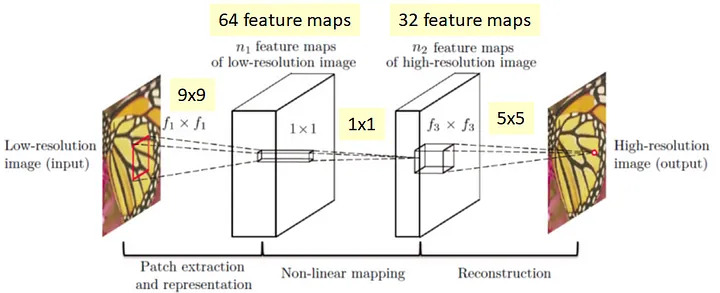
\includegraphics[width=5in]{./figures/srcnn.jpg}
        \caption{SRCNN Representation}
    \end{figure}
\end{enumerate}
\newpage
\section{FEASIBLITY ANALYSIS}
We are planning to use deep learning to develop a system that can increase the
resolution of image. The system is trained on dataset of high-resolution images and
low-resolution images generated using degradation model to generate high resolution
images from low resolution images.\\
Deep learning is shown to be very effective for ISR. There are many models
developed for this task we can take inspiration from. The technical feasibility of this
project is therefore high. The cost of developing the system will depend on the size of
the dataset used to train the model, and the complexity of the model. As we are planning
to train the model on server and deploy the system on cloud-based service. So, server
costs will be our main cost for this project. \\
The technical and economic feasibility analysis show that we can complete this
project successfully. 
\newpage
\section{RESULT AND DISCUSSION}
\subsection{Work Completed}
\subsection{Work Remaining}
\subsection{Limitations}
\subsection{Problem Faced}
\subsection{Budget Analysis}
\subsection{Work Schedule}
% \bibliographystyle{apalike}
\newpage
\bibliographystyle{unsrt}
\bibliography{sections/references.bib}

\end{document}